\documentclass[11pt]{article}
\raggedbottom

% NeurIPS 2024 style
\usepackage[preprint]{neurips_2024}

% Packages
\usepackage[utf8]{inputenc}
\usepackage{amsmath,amssymb,amsfonts}
\usepackage{graphicx}
\usepackage{booktabs}
\usepackage{array}
\usepackage{hyperref}
\usepackage{xcolor}
\usepackage{fontspec}
\setmainfont[
  BoldFont={Noto Sans KR},
  BoldFeatures={Weight=700},
  ItalicFont={Noto Sans KR},
  Scale=0.97
]{Noto Sans KR}
\setsansfont[Scale=0.97]{Noto Sans KR}

\hypersetup{
  colorlinks=true,
  linkcolor=black,
  citecolor=black,
  urlcolor=black
}

% Spacing overrides
\emergencystretch=2em
\setlength{\parskip}{3pt plus 1pt minus 1pt}
\setlength{\floatsep}{8pt plus 2pt minus 2pt}
\setlength{\textfloatsep}{10pt plus 3pt minus 3pt}
\setlength{\intextsep}{8pt plus 2pt minus 2pt}
\setlength{\abovecaptionskip}{4pt}
\setlength{\belowcaptionskip}{2pt}
% Section heading spacing
\makeatletter
\renewcommand\section{\@startsection{section}{1}{\z@}%
  {-18pt \@plus -4pt \@minus -2pt}%
  {6pt \@plus 2pt}%
  {\normalfont\large\bfseries}}
\renewcommand\subsection{\@startsection{subsection}{2}{\z@}%
  {-12pt \@plus -2pt \@minus -2pt}%
  {4pt \@plus 1pt}%
  {\normalfont\normalsize\bfseries}}
\renewcommand\subsubsection{\@startsection{subsubsection}{3}{\z@}%
  {-6pt \@plus -1pt \@minus -1pt}%
  {2pt}%
  {\normalfont\normalsize\itshape}}
\makeatother

% Custom commands
\newcommand{\sgmvpi}{$(S, G, E, V, M, \pi)$}
\newcommand{\framework}{\textsc{SciAgent}}

% Title
\title{\textbf{AI 과학자 시스템의 형식화:\\
자동화된 과학적 발견을 위한 통합 프레임워크}}

\author{
  Jaesol Shin\\
  \small{WeDataLab}\\
  \texttt{ysys143@wedatalab.com}
}

\date{2026년 5월}

\begin{document}

\maketitle

\begin{abstract}
가설 생성, 실험 실행, 지식 합성을 자동화하는 엔드투엔드 시스템의 등장은 과학이 수행되는 방식에 중대한 변화를 가져오고 있다. 빠른 경험적 발전에도 불구하고, \emph{AI 과학자} 시스템들은 통합된 형식 프레임워크가 없어 아키텍처 및 과학 도메인 간 원칙적 비교가 어렵다. 본 논문은 \framework{}, 즉 탐색 공간(\textbf{S}earch space), 가설 생성기(hypothesis \textbf{G}enerator), 실험 실행기(\textbf{E}xperiment executor), 검증기(\textbf{V}alidator), 메모리(\textbf{M}emory), 탐색 정책(search \textbf{P}olicy, $\pi$)의 여섯 구성요소로 이루어진 프레임워크 \sgmvpi{}를 제안한다. 이 프레임워크는 부분 관측 마르코프 결정 과정(POMDP) 이론과 베이즈 실험 설계(BED) 이론에 기반한다. 본 논문은 핵심 AI 과학자 시스템 및 일곱 개 과학 도메인(수학, 물리학, 화학, 재료과학, 생물학, 사회과학, 컴퓨터 과학)에 걸친 구체적 적용을 분석하고, 이러한 시스템의 출력 형식과 검증 계층을 다루는 상호 보완적인 아티팩트 인프라 제안도 별도로 검토한다. 분석을 통해 세 가지 지속적인 미해결 문제가 도출된다: (1) 신규성 평가의 자동화 불가능성---다층적 자동화 프록시에도 불구하고 인간 판단에 여전히 의존; (2) BED 최적 탐색 정책의 부재---실현 가능한 근사 방법이 이론적으로 존재함에도 불구하고; (3) 의미 메모리 $M_s$의 미성숙---축적된 실험 경험이 미래 탐색을 개선하지 못하는 문제. 본 논문은 검증기 $V$의 완결성이 설계 변수 중 가장 중요한 단일 변수임을 보인다: 각 도메인에서 폐루프 자율 운영의 가능 여부를 결정하며, 현재 AI 과학자 시스템들은 더 완전한 검증기를 향한 진행으로 해석할 수 있다.
\end{abstract}

\section{서론}

AI 과학자 시스템---가설을 독립적으로 생성하고, 실험을 실행하며, 지식을 합성하는 에이전트---은 급속도로 증가하고 있으나~\citep{boiko2023emergent,lu2024aiscientist,lu2026aiscientist,schmidgall2025agentlab,google2026aletheia,liu2026lasthuman}, 이 분야는 공통된 형식 어휘가 부재하다. 각 시스템은 고유한 용어를 도입하여 체계적인 비교를 어렵게 한다. 실제 배포에 직결되는 세 가지 질문이 여전히 미답 상태이다: \textit{어떤 요소가 시스템의 폐루프 운영 가능 여부를 결정하는가? 자율적 신규성 평가는 왜 지속적으로 실패하는가? 이론적으로 최적인 탐색 정책은 무엇인가?}

본 논문은 세 가지 기여로 이 격차를 해소한다: (1)~\framework{}, AI 과학자 시스템을 POMDP 및 베이즈 실험 설계 이론과 연결하는 형식 프레임워크 \sgmvpi{} (§\ref{sec:framework}); (2)~네 개의 핵심 시스템, 아티팩트 인프라 제안, 그리고 일곱 개 과학 분야에 걸친 도메인별 구체화 분석 (§\ref{sec:core}, §\ref{sec:domains}); (3)~모든 현재 시스템에 걸쳐 진전을 제약하는 세 가지 미해결 문제 (§\ref{sec:openproblems}).

\noindent\textbf{범위.} 본 논문은 가설-실험-검증 주기를 통해 과학적 \emph{발견}을 자동화하는 것이 주된 목표인 시스템을 다루며, 인간 주도 파이프라인 내 특화 도구~\citep{jumper2021alphafold}는 제외한다.

\section{배경}
\label{sec:background}

\citet{kaelbling1998pomdp}의 POMDP 정식화에 따라, AI 과학자 시스템을 \emph{부분 관측 마르코프 결정 과정}으로 모델링한다: 진상태 $s$(자연의 미지 구조)는 직접 접근 불가능하며; 시스템은 실험적 관측으로 업데이트되는 믿음 상태 $b(s)$를 유지한다. 형식적으로, AI 과학자 POMDP는 튜플 $(\mathcal{S}, \mathcal{A}, T, R, \Omega, \mathcal{O})$이며, 여기서 $\mathcal{A}$는 행동 공간(가설 생성 및 실험 실행), $T$는 전이 함수, $R$은 보상(발견의 과학적 가치), $\mathcal{O}$는 잡음이 있는 관측 과정이다. 세 가지 속성이 표준 제어 문제와 구별한다: $R$은 사전에 명시될 수 없다(유의성은 선험적으로 정의되지 않음); $\mathcal{S}$는 무한하다; $T$는 비정상적이다(축적된 지식이 탐색 전선을 변화시킴). 베이즈 실험 설계(BED)~\citep{chaloner1995bayesian,rainforth2024modern}는 탐색 정책 $\pi$의 규범적 기준을 제공한다: 기대 정보 이득(EIG)을 최대화하는 $d^*$를 선택하고,

\begin{equation}
  d^* = \arg\max_{d \in \mathcal{D}}\; \mathrm{EIG}(d) = \arg\max_{d}\; \mathbb{E}\left[H(\theta) - H(\theta \mid y, d)\right]
  \label{eq:eid}
\end{equation}

여기서 $H(\theta)$는 매개변수 $\theta$에 대한 사전 엔트로피이고, $H(\theta \mid y, d)$는 $d$ 하에서 $y$를 관측한 후의 기대 사후 엔트로피이다. EIG는 변분 방법~\citep{foster2019variational}, 분할 상환 정책~\citep{foster2021dad}, 강화학습~\citep{blau2022rl}으로 근사할 수 있으나, 현재 어떤 AI 과학자 시스템도 이를 구현하지 않는다---§\ref{sec:openproblems}에서 다루는 격차이다.

\section{관련 연구}
\label{sec:related}

\textbf{AI 과학자 시스템.} 선행 연구~\citep{lu2024aiscientist,lu2026aiscientist,schmidgall2025agentlab,boiko2023emergent}는 개별 시스템에 대한 정성적 특성화를 제공하지만 교차 시스템 비교를 위한 공통 프레임워크는 없다; 아이디어 생성 연구~\citep{si2024novelideas,baek2024researchagent}는 완전한 발견 루프를 통합하지 않은 채 품질 기준선을 수립한다.

\textbf{이론적 기반.} POMDP 프레임워크~\citep{kaelbling1998pomdp}와 BED~\citep{chaloner1995bayesian,rainforth2024modern}는 고전적이다; 본 논문은 BED를 AI 과학자 탐색 정책의 설계 목표로 명시적으로 적용한 최초의 연구로, POMDP(구조적 정식화)와 BED(규범적 정책 기준)를 연결한다.

\textbf{과학의 형식 모델과 아티팩트 인프라.} \citet{taniguchi2024cpc}는 집합적 예측 코딩을 과학의 사회적 모델로 제안한다; 본 논문은 상호 보완적인 단일 시스템 모듈형 분해를 제공한다. \citet{liu2026lasthuman}은 §\ref{sec:ara} 및 §\ref{sec:openproblems}에서 논의되는 $V$ 및 $M_s$ 기여로서 아티팩트 검증을 다룬다.

\section{\framework{} 프레임워크}
\label{sec:framework}

AI 과학자 시스템을 다음 구성요소를 가진 튜플 \sgmvpi{}로 정의한다:

\begin{equation}
  \text{\framework{}} = (S,\; G,\; E,\; V,\; M,\; \pi)
\end{equation}

\begin{description}
  \item[$S$: 탐색 공간 (Search Space)] 탐색 대상인 후보 가설, 프로그램, 분자, 실험 조건 또는 기타 객체의 집합. $S$는 정적이거나 동적으로 확장(개방형)될 수 있다.

  \item[$G: M \times S \rightarrow h$: 가설 생성기 (Hypothesis Generator)] 축적된 메모리 $M$과 탐색 공간의 현재 상태를 조건으로 새로운 후보 $h \in S$를 제안하는 함수. $G$는 LLM 생성, 진화적 돌연변이, 또는 기호적 탐색을 수반할 수 있다.

  \item[$E: h \times P \rightarrow o$: 실험 실행기 (Experiment Executor)] 프로토콜 $P$ 하에서 가설 $h$를 실행하여 관측 $o$를 생성하는 함수. $E$의 충실도는 빠른 계산 시뮬레이션(낮은 비용, 잠재적 대리 오차)에서 물리적 습식 실험실 실행(높은 비용, 실제 정답)까지 다양하다.

  \item[$V: o \rightarrow r$: 검증기 (Validator)] 관측 $o$에 보상 신호 $r$을 할당하는 함수. $V$의 네 계층을 구별한다:
    \begin{align*}
      V_\text{syntax}   &: o \rightarrow \{\text{pass}, \text{fail}\} & \text{(결정론적, 고속)}\\
      V_\text{semantic} &: o \rightarrow r \in [0,1]                  & \text{(LLM 기반, 확률적)}\\
      V_\text{empirical}&: o \rightarrow r                            & \text{(재현 기반)}\\
      V_\text{human}    &: o \rightarrow \{\text{novel}, \text{significant}\} & \text{(자동화 불가)}
    \end{align*}

  \item[$M$: 메모리 (Memory)] $(M_e, M_s, M_p)$로 구성. $M_e$(일화)는 개별 기록 $(h_i, o_i, r_i)$를 저장; $M_s$(의미)는 증류된 지식 패턴을 저장; $M_p$(절차)는 학습된 프로토콜을 저장. $M$의 구조는 $G$와 $\pi$의 품질을 직접 결정한다.

  \item[$\pi: b(S) \times M \rightarrow h$: 탐색 정책 (Search Policy)] 다음 가설을 선택하는 결정 규칙. 믿음 상태 $b(S)$는 각 실험 후 업데이트된다. BED 해석에서 $\pi^* = \arg\max_d \mathrm{EIG}(d)$ (식~\ref{eq:eid}). 실제로는 반응형(ReAct)에서 탐욕적, 트리 탐색까지 다양한 정책이 사용된다.
\end{description}

\noindent 운영 루프는 다음과 같다:
\begin{align}
  \pi(b, M) &\;\rightarrow\; G(M_s, S) \;\rightarrow\; E(h, P) \;\rightarrow\; V(o) \nonumber\\
            &\;\rightarrow\; M \mathrel{+}= (h, o, r) \;\rightarrow\; b(S) \text{ 업데이트} \;\rightarrow\; \text{반복}
\end{align}

인간 개입 정도를 나타내는 보조 매개변수 $H \in [0,1]$을 추가로 도입한다: $H=0$은 완전 자율 시스템, $H=1$은 인간이 $G$ 또는 $\pi$의 역할을 맡는 시스템이다.

\section{핵심 AI 과학자 시스템 분석}
\label{sec:core}

\framework{}를 네 개의 엔드투엔드 시스템~\citep{boiko2023emergent,lu2024aiscientist,lu2026aiscientist,schmidgall2025agentlab}과 하나의 아티팩트 인프라 제안에 적용한다. 표~\ref{tab:core-comparison}은 핵심 차원을 종합한다; 시스템 간 공통 패턴은 모든 아키텍처적 발전이 $V$ 완결성의 향상이며, $V$ 완결성이 폐루프 운영을 가능하게 한다는 것이다.

\vspace{6pt}
\begin{table}[h]
\centering
\small
\setlength{\tabcolsep}{4pt}
\begin{tabular}{@{}lcccc@{}}
\toprule
& \textbf{Coscientist} & \textbf{AI Sci.\ (2024)} & \textbf{AI Sci.\ (2026)} & \textbf{AgentLab} \\
\midrule
신규성 측정    & 없음         & LLM 자체 평가  & 3단계           & 인간 위임       \\
루프 폐쇄?     & 아니오       & 예(탐욕적)     & 예(트리)        & 부분적          \\
$\pi$ 유형     & ReAct        & 탐욕적         & 트리 탐색       & 인간/순차        \\
$V$ 완결성     & $V_h$ 전용   & $V_s$          & $V_e+V_s+V_h$  & $V_s$ (편향)    \\
$M$ 구조       & 일시적       & $M_e$          & $M_e+M_s$       & $M_e$           \\
$H$ (인간 역할) & G            & 낮음           & 낮음            & G+$\pi$         \\
\bottomrule
\end{tabular}
\caption{네 핵심 AI 과학자 시스템의 비교 \framework{} 분석. $V_s$=의미, $V_e$=실증, $V_h$=인간.}
\label{tab:core-comparison}
\end{table}

\subsection{아티팩트 인프라: 에이전트 네이티브 연구 아티팩트}
\label{sec:ara}

\citet{liu2026lasthuman}은 상호 보완적인 문제를 다룬다: AI 과학자 루프의 \emph{출력}이 어떤 모습이어야 하는지, 그리고 독립적으로 어떻게 검증될 수 있는지. 에이전트 네이티브 연구 아티팩트(ARA)는 서사적 논문을 네 계층의 온톨로지로 대체한다: \texttt{/logic}(반증 기준이 있는 주장), \texttt{/src}(실행 가능 코드), \texttt{/trace}(탐색 그래프: 질문, 결정, 실험, 막다른 길, 전환), \texttt{/evidence}(원시 결과). ARA 씰은 세 단계 자동 검증을 제공한다---$V_\text{syntax}$(스키마 적합성), $V_\text{semantic}$(엄격성 감사기, 82.6\% 탐지율), $V_\text{empirical}$(샌드박스 재현)---$V_\text{human}$은 유의성, 신규성, 취향을 위해 명시적으로 유보된다: \textit{``유의성, 신규성, 취향에 대한 판단은 인간 심사위원을 위해 유보된다''}~\citep{liu2026lasthuman}. 동기는 정량적이다: 출판 논문의 재현 요건 중 45.4\%만이 완전히 명시되어 있고, 확장 비용의 90.2\%는 실패한 탐색에 소비된다~\citep{liu2026lasthuman}. \texttt{/trace} 계층은 $M_e$와 $M_s$를 다룬다: 보존된 실패 흔적은 에이전트의 확장 과업 성능을 가속화하지만, 동시에 더 유능한 에이전트를 이전 해결 경로에 고착시켰다---풍부한 $M_e$가 $\pi$를 단조적으로 개선하지 않는다.

\section{도메인 분석}
\label{sec:domains}

표~\ref{tab:domain-comparison}은 일곱 개 과학 도메인에 걸친 \framework{} 구체화를 보여준다; $V$ 완결성은 예외 없이 루프 폐쇄 가능성과 공변한다. 규모를 예시하면: Aletheia~\citep{google2026aletheia}는 700개의 에르되시 문제를 시도했으며, 심사위원은 200개 채점 해법 중 13개(6.5\%)를 의미있게 정확하다고 평가했다; GNoME~\citep{merchant2023gnome}은 고처리량 DFT를 통해 220만 개의 후보 결정 구조를 검토했다. 분석 대상 시스템: 수학(형식적:~\citep{romera2023funsearch,xin2024deepseek}; 자연어:~\citep{google2026aletheia}), 물리학~\citep{udrescu2020afeynman,cranmer2020symbolic}, 화학~\citep{bran2023chemcrow,sprueill2024chemreasoner}, 재료과학~\citep{merchant2023gnome}, 생물학~\citep{odonoghue2023bioplanner}, 사회과학~\citep{manning2024automated,aher2023turing,park2023generative}, 컴퓨터 과학/알고리즘~\citep{real2020automlzero,sartori2024algodiscovery,jaber2026autokernel}.

\begin{table}[h]
\centering
\small
\setlength{\tabcolsep}{4pt}
\begin{tabular}{@{}lccccp{2.6cm}@{}}
\toprule
도메인 & $V$ 유형 & $V$ 신뢰도 & 루프 & $\pi$ & 주요 병목 \\
\midrule
수학(형식) & $V_\text{formal}$ & 완벽 오라클 & 완전 폐쇄 & RL/MCTS  & 사전훈련 오염 \\
수학(자연어) & $V_\text{sem}+V_h$ & 불완전 & 부분적 & 순차 개선 & 환각; 표절 \\
물리학 & $V_\text{emp}+V_h$ & 중간 & 없음/부분적 & 결정론적 & 문제 간 $M$ 없음 \\
화학 & $V_\text{emp}$ (대리) & 중간 & 계산만 & 빔 탐색 & 습식 루프 개방 \\
재료과학 & $V_\text{emp}$ (DFT) & 높음 & 계산 폐쇄 & 불확실성 샘플링 & DFT 연산 시간; 합성 지연 \\
생물학 & $V_\text{emp}+V_h$ & 낮음--중간 & 부분적 & 없음 & $V$ 지표 불충분 \\
사회과학 & 통계 검정 & 낮음--중간 & 부분적 & 완전 요인 & 순환 타당성 \\[3pt]
CS/알고리즘 & $V_\text{emp}$ & 높음 & 완전 폐쇄 & 진화/LLM & 해석 가능성 부재 \\
\bottomrule
\end{tabular}
\caption{일곱 개 도메인에 걸친 \framework{} 교차 도메인 분석. $V$ 신뢰도는 실제 정답과의 일치도를 나타낸다.}
\label{tab:domain-comparison}
\end{table}

\noindent 도메인 패턴은 우연이 아니다. 수학(형식)에서, 잡음 없는 $V_\text{formal}$은 안정적인 강화학습을 가능하게 한다: 이진적이고 명확한 보상은 해킹될 수 없다. 화학과 생물학에서, 자동화된 $V$가 물리적 측정(NMR, MS, 습식 실험실 검증)을 대체할 수 없기 때문에 루프가 폐쇄될 수 없다. 재료과학은 $\pi$가 BED 이론에 가장 근접한 유일한 도메인이다: 추적 가능한 GNN 사후 확률에 대한 GNoME의 불확실성 샘플링이 EIG 최적 탐색에 가장 가까운 현존 배포이다. 사회과학은 별개의 실패 양식에 직면한다: $G$와 $E$가 동일한 기반 모델을 공유할 때, 평가자는 생성기의 암묵적 편향을 체계적으로 확인한다~\citep{aher2023turing}.

% ---------------------------------------------------------------------------
\section{예시 시뮬레이션: 검증기 커버리지와 허위 신규성}
\label{sec:simulation}
% ---------------------------------------------------------------------------

$V$ 불완결성의 결과를 구체화하기 위해, 에이전트가 커버리지 멤버십 검사로 신규성을 추정하고 통신 토폴로지(주된 독립변수)를 통해서만 메모리를 공유하는 최소 에이전트 기반 시뮬레이션(20 에이전트, 200 가설, 40 잠재 클래스, 30 시드)을 실행한다. 표~\ref{tab:sim-conditions}은 네 조건을 $V$ 완결성의 수준으로 형식화한다.

\begin{table}[h]
\centering
\small
\caption{시뮬레이션 조건. 각 조건은 평균 차수 $k$를 통해 $V$ 완결성의 수준을 조작화한다.}
\label{tab:sim-conditions}
\begin{tabular}{@{}lllll@{}}
\toprule
조건 & $V$ 완결성 & $k$ & 그래프 & 커버리지 \\
\midrule
고립     & 불완전     & 0   & 간선 없음       & 자체 메모리만 \\
격자     & 부분적     & 2   & 링              & 2-홉 이웃 \\
중간     & 개선됨     & 4   & Watts--Strogatz & 지역 + 교차 연결 \\
공유     & 완전       & $n{-}1$ & 완전 그래프 & 전체 커뮤니티 메모리 \\
\bottomrule
\end{tabular}
\end{table}

\textbf{결과.} 그림~\ref{fig:fnr}은 조건 간 허위 신규성 비율(FNR: 신규하지 않은 가설이 신규로 표시되는 비율)을 보여준다. 메모리 공유가 집합-합집합(set-union)이므로, 더 넓은 연결성은 구조적으로 FNR을 감소시킨다---이는 창발적 발견이 아닌 메커니즘의 분석적 결과이다. FNR은 $0.955 \pm 0.028$(고립)에서 $0.008 \pm 0.012$(공유)로 감소한다; 분류기 정확도 0.60--0.90 변화는 FNR을 $\leq 0.035$ 이동시켜, 이는 교차 토폴로지 폭의 $27$배 더 작은 범위이다. $\geq 10\%$ 사전 시딩에서 비자명한 결과가 나타난다: 고립 에이전트가 격자보다 \emph{더 높은} 균형 정확도를 달성한다($0.564$ 대 $0.529$). 인식론적 네트워크 모델~\citep{zollman2007communication,zollman2010epistemic}과의 유사성은 현상론적 수준에서만 성립한다.

\begin{figure}[h]
\centering
\vspace{4pt}
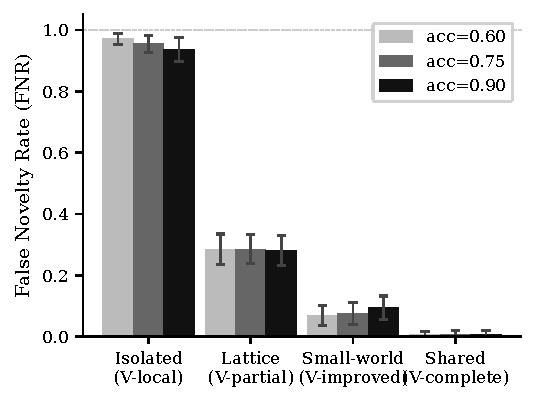
\includegraphics[width=0.65\columnwidth]{fig_fnr_primary_n30.pdf}
\vspace{4pt}
\caption{$V$ 완결성 수준 및 분류기 정확도별 FNR ($\pm 1$ 표준편차, 30 시드). 교차 토폴로지 폭: $0.947$; 조건 내 정확도 범위: $\leq 0.035$.}
\label{fig:fnr}
\end{figure}

\textbf{한계.} 실제 정답 오라클이 있는 합성 에이전트; 에이전트는 가설을 생성하거나 믿음을 업데이트하지 않는다. 시뮬레이션은 $V$ 불완결성의 존재 예시이다---FNR-토폴로지 순서는 구조적으로 결정되어 다른 결과를 생성할 수 없다.

\section{미해결 문제}
\label{sec:openproblems}

본 분석은 모든 시스템과 도메인에 걸쳐 지속되는 세 가지 미해결 문제를 식별한다.

\subsection{신규성의 자동화 불가능성}

신규성은 자동화된 수단으로 신뢰할 수 있게 평가될 수 없다: Coscientist(메커니즘 없음)에서 The AI Scientist Nature(3단계 검증)까지 모든 시스템이 이 결론으로 수렴한다. 두 가지 실패 양식이 문서화되어 있다: LLM 자체 평가 편향(체계적 과대 추정; 환각된 결과)과 사전훈련 오염(시스템이 훈련 데이터에 암묵적인 결과를 ``발견''할 수 있음, Aletheia가 에르되시 문제에서 문서화한 것처럼). ARA 씰~\citep{liu2026lasthuman}은 자동화 전선을 표시한다---5개 주입 유형에 걸쳐 구조적 위반의 82.6\% 탐지, 고아 실험에 대한 22\% 맹점---그러나 신규성 경계를 넘을 수 없다. 구체적으로: Agent Laboratory의 LLM 심사위원은 평균 $+$2.3점을 과대 추정했고; The AI Scientist(Sakana)는 절제 실험 표를 환각했으며; Aletheia는 700개의 에르되시 문제를 심사하여 표면적으로 그럴듯한 많은 후보에도 불구하고 채점된 해법 중 6.5\%만이 의미있게 정확하다는 것을 발견했다.

\textit{반증 기준:} 자동화된 $V$가 $\geq$3개 과학 도메인에 걸친 오염-통제 벤치마크에서 인간 수준의 신규성 판별(평가자 간 일치도 $\geq$0.80)을 달성하면 반증된다.

\subsection{$\pi$의 BED--실제 격차}

식~\ref{eq:eid}은 이론적으로 최적인 정책을 명시하지만, 현재 어떤 시스템도 이를 구현하지 않는다: 모든 배포 정책은 휴리스틱이다(ReAct, 탐욕적, 트리 탐색, 인간 주도). 부분적 예외는 GNoME~\citep{merchant2023gnome}으로, 추적 가능한 GNN 사후 확률에 대해 EIG를 근사하는 심층 앙상블 불확실성 샘플링을 사용한다---그러나 이는 DFT가 잘 보정된 $V$를 제공하고 가설 공간이 학습 가능한 확률 모델을 허용하기 때문이며, LLM 기반 시스템에는 없는 조건으로 ``사후 확률''이 모델 가중치에 암묵적으로 존재한다~\citep{foster2021dad}. 구체적으로, 표~\ref{tab:core-comparison}의 모든 시스템은 휴리스틱 $\pi$로 저하된다: Coscientist는 반응적으로 다음 도구를 선택하고, The AI Scientist(Sakana)는 탐욕적으로 아카이브 유사성을 회피하며, Agent Laboratory는 고정된 순차 스케줄을 따른다---어떤 것도 추가 실험 데이터로 개선되지 않으며, 이것이 EIG 최적 $\pi$가 피할 실패 양식이다.

\textit{반증 기준:} 사후 확률이 제1원리로 추적 가능하지 않은 도메인에서 $p(\theta \mid y)$에 대한 사후 확률을 명시적으로 계산하고 EIG를 최대화하는 정책을 구현하는 AI 과학자 시스템이 있으면 반증된다---GNoME의 심층 앙상블 정책과 같은 추적 가능 모델 프록시는 제외한다.

\subsection{의미 메모리 $M_s$의 미성숙}

현재 시스템들은 원시 실험 기록($M_e$)을 저장하지만 전이 가능한 패턴($M_s$)으로 증류하지 않는다: 1,000개의 실험을 가진 시스템은 10개를 가진 시스템보다 더 지능적으로 탐색하지 않는다. ARA \texttt{/trace} 계층~\citep{liu2026lasthuman}이 가장 가까운 근사이지만, 흔적은 확장 과업 성능을 가속화하는 동시에 유능한 에이전트를 이전 해결 경로에 고착시켰다---$M_s$ 구조는 선택적 망각 메커니즘과 결합되어야 유익하다. 구체적으로, GNoME의 GNN---$G(M_s, S)$가 진정으로 개선되는 몇 안 되는 시스템 중 하나---은 460K DFT 계산 후 도메인별 열역학 지식을 축적하지만, 이 지식은 화학이나 생물학으로 전이되지 않는다; 명시적으로 훈련하지 않은 도메인에서는 더 유능하지 않다.

\textit{반증 기준:} 사전에 지정된 지표로 측정하여, 축적된 교차 실험 지식이 단일 도메인 내 과업 인스턴스에 걸쳐 $G$ 생성 가설의 품질을 입증 가능하게 개선하면 반증된다.

\noindent 세 미해결 문제는 독립적이지 않다. 완전한 $V$와 추적 가능한 $M_s$를 가진 시스템은 구성적으로 EIG 최적 $\pi$를 구현할 수 있을 것이다: 완전한 $V$는 보정된 해킹 불가능 보상 신호를 제공하고, 발전된 $M_s$는 EIG가 요구하는 가설 공간 모델을 유지한다. 따라서 이들은 단일 구조적 격차로 수렴하며, 어느 하나에서의 진전은 다른 둘에 대한 불균형적인 이득을 잠금해제한다. 이들은 또한 집합적 AI 공동 과학자~\citep{taniguchi2024cpc}의 실현에 필요한 조건이기도 하다: $V_\text{collective}$는 신규성 자동화 가능성 해결을 요구하고; 원칙적인 집합 $\pi$는 BED--실제 격차 해소를 요구하며; 공유 의미 메모리 $w$는 발전된 $M_s$를 요구한다. ARA~\citep{liu2026lasthuman}은 $M_s$를 외재화하고 $V$의 신규성 경계 이하 계층을 보정함으로써 두 문제를 동시에 다루는 가장 실현 가능한 진입점일 수 있다.

\section{논의}
\label{sec:discussion}

본 분석은 설계 위계를 확립한다: $V$ 선택이 모든 다른 결정보다 선행하며, 폐루프 가능성과 $\pi$가 취할 수 있는 형태를 결정한다. 집합적 확장~\citep{taniguchi2024cpc}은 세 미해결 문제가 먼저 해결될 것을 요구한다: $V_\text{collective}$는 신규성 자동화 가능성을 요구하고; 원칙적인 집합 $\pi$는 BED--실제 격차 해소를 요구하며; 발전된 $M_s$는 공유 의미 메모리 $w$를 가능하게 한다. ARA~\citep{liu2026lasthuman}은 $w$를 위한 구조적 아티팩트 프로토콜로서 가장 실현 가능한 진입점일 수 있다. 한계: \framework{}은 $E$의 도메인 특화 비용 구조(도메인에 따라 수십 배 차이), $S$의 비정상성(개방형 문제), 그리고 \citet{taniguchi2024cpc}가 형식화한 사회적 계층을 추상화한다.

\section{결론}
\label{sec:conclusion}

본 논문은 AI 과학자 시스템을 POMDP 및 BED 이론과 연결하는 형식 프레임워크인 \framework{} \sgmvpi{}를 도입하고, 이를 네 개의 핵심 시스템, 하나의 아티팩트 인프라 제안, 일곱 개 과학 도메인에 적용했다. 핵심 발견은 $V$ 완결성이 폐루프 가능성의 주된 결정 변수라는 것이다: 조사된 시스템 전반에 걸쳐 모든 아키텍처적 발전은 궁극적으로 $V$ 완결성의 향상이다. 세 미해결 문제---신규성 자동화 불가능성, BED--실제 격차, $M_s$ 미성숙---는 단일 조직화 질문으로 수렴한다: \textit{폐루프 운영을 지원하기에 충분히 완전하면서 원칙적인 탐색을 지원하기에 충분히 구조화된 검증기와 메모리 구조를 어떻게 구축할 것인가?}

\bibliographystyle{abbrvnat}
\bibliography{references}

\newpage
\section*{AI 참여 체크리스트}
\label{sec:ai-checklist}

이 체크리스트는 CAISc 2026이 요구하는 대로 이 연구의 각 단계에서 AI 시스템의 역할을 문서화한다.

\begin{itemize}
  \item \textbf{가설 개발.} 핵심 \framework{} 프레임워크 \sgmvpi{}, $H$ 매개변수, $G$ 출력 스펙트럼(명제 가설 $\to$ 반증 가능한 구성), 세 가지 미해결 문제는 인간 저자가 구상했다. Claude Code(Anthropic)는 프레임워크 구성요소를 정교화하고, 각 구성요소의 논문 수준 구체화를 식별하며, 개념 간 연결을 제안했다.

  \item \textbf{문헌 검색 및 선택.} 인간 저자가 포함 기준과 대상 시스템을 결정했다. Claude Code는 자율적으로 40개 이상의 전문 PDF를 검색, 열람하고, 논문들을 분류학으로 범주화하며, 원문 대비 주장 수준의 검증을 수행했다.

  \item \textbf{분석.} Claude Code는 1차 자료를 읽어 13개 분석 시스템 각각의 S, G, E, V, M, $\pi$ 구성요소를 추출했다. 인간 저자는 모든 추출을 검토하고, 오류를 수정(여러 실질적 수정이 필요했음)하며, 교차 시스템 패턴을 종합했다.

  \item \textbf{작성.} Claude Code가 이 원고의 대부분을 초안 작성했다. 인간 저자는 핵심 개념적 단락(특히 §\ref{sec:openproblems} 및 §\ref{sec:framework}의 핵심 정의)을 제공하고, 구조적 결정을 지시하며, 모든 초안을 검토했다.
\end{itemize}

\noindent 전반적으로, 분업의 특성은 다음과 같다: 인간 저자는 지적 방향, 프레임워크 설계, 최종 판단을 제공했고; Claude Code는 문헌 검색, 분석 실행, 텍스트 생성을 담당했다.

% ---------------------------------------------------------------
\newpage
\section*{책임 및 재현성 체크리스트}
\label{sec:repro-checklist}

\begin{itemize}
  \item \textbf{주장과 증거.} 모든 경험적 주장은 인용된 1차 자료에 근거한다. 주요 주장은 원본 PDF의 직접 전문 열람으로 검증되었다.

  \item \textbf{한계.} 이 논문은 기존 출판 시스템의 개념적 메타 분석이다. 독창적인 실험을 포함하지 않는다. \framework{} 프레임워크는 이 제출에서 보류 시스템에 대해 경험적으로 검증되지 않았으며; 기술적 적절성은 분석된 13개 시스템 전반의 일관성에 달려있다.

  \item \textbf{재현성.} \framework{}은 구성요소 정의에 따라 어떤 AI 과학자 시스템에도 적용될 수 있다. 분석된 모든 논문은 공개적으로 접근 가능하다. 독점 데이터나 비공개 모델은 사용되지 않았다.

  \item \textbf{실험 세부사항.} 문헌 검토 방법론은 Muka et al.\ (2020) 24단계 체계적 검토 지침을 따른다. 시스템 선택 기준: 가설--실험--검증 루프의 최소 하나의 구성요소를 자동화한다.

  \item \textbf{데이터 및 코드 가용성.} 분석 노트는 채택 시 공개될 것이다. 데이터셋은 생성되지 않았다.

  \item \textbf{윤리적 및 사회적 영향.} $H$ 매개변수 분석은 현재 시스템에서 인간 감독의 필요성을 명시적으로 다룬다. §\ref{sec:openproblems}의 미해결 문제 논의는 AI 과학자 광범위 배포 하의 조기 수렴 위험을 식별하며, 특히 $M_s$ 미성숙 문제를 통해.
\end{itemize}

\end{document}
